% Circular arrows with text
% Author: Tom Bombadil
% https://texample.net/tikz/examples/circular-arrows-text/
\documentclass[tikz,border=10pt]{standalone}
\usetikzlibrary{decorations.text}
\newcommand*{\mytextstyle}{\sffamily\Large\bfseries\color{black!85}}
\newcommand{\arcarrow}[8]{%
% inner radius, middle radius, outer radius, start angle,
% end angle, tip protusion angle, options, text
  \pgfmathsetmacro{\rin}{#1}
  \pgfmathsetmacro{\rmid}{#2}
  \pgfmathsetmacro{\rout}{#3}
  \pgfmathsetmacro{\astart}{#4}
  \pgfmathsetmacro{\aend}{#5}
  \pgfmathsetmacro{\atip}{#6}
  \fill[#7] (\astart:\rin) arc (\astart:\aend:\rin)
       -- (\aend+\atip:\rmid) -- (\aend:\rout) arc (\aend:\astart:\rout)
       -- (\astart+\atip:\rmid) -- cycle;
  \path[font = \sffamily, decoration = {text along path, text = {|\mytextstyle|#8},
    text align = {align = center}, raise = -0.5ex}, decorate]
    (\astart+\atip:\rmid) arc (\astart+\atip:\aend+\atip:\rmid);
}

\begin{document}
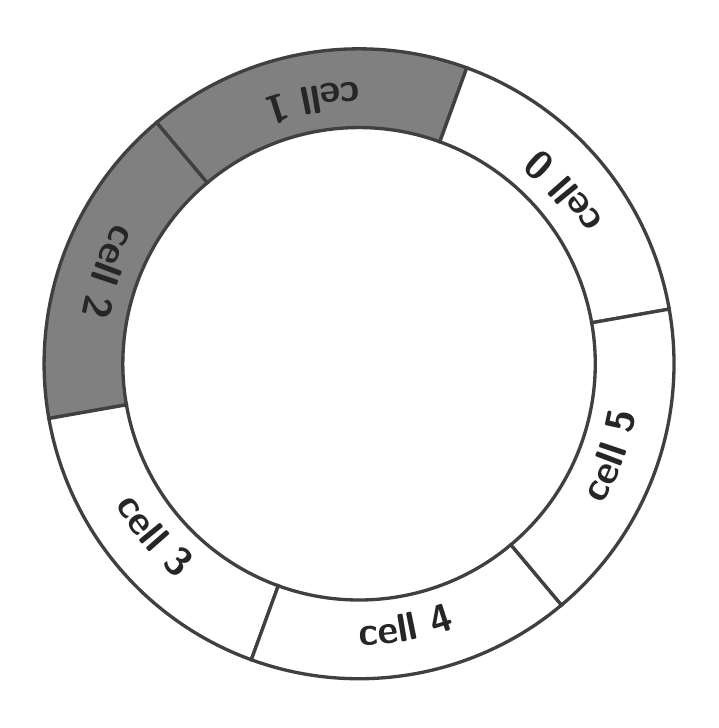
\begin{tikzpicture}
  %\fill[even odd rule,red!30] circle (3.8) circle (3.2);
  %\foreach \x in {0,1,...,5} {
  %  \arcarrow{3}{3.5}{4}{\x*60+10}{\x*60+70}{0}{gray,
  %    draw = gray!50!black, very thick}{cell \x}
  %}
  \foreach \x in {1,2} {
    \arcarrow{3}{3.5}{4}{\x*60+10}{\x*60+70}{0}{gray,
      draw = gray!50!black, very thick}{cell \x}
  }
  \foreach \x in {0,3,4,5} {
    \arcarrow{3}{3.5}{4}{\x*60+10}{\x*60+70}{0}{white,
      draw = gray!50!black, very thick}{cell \x}
  }

\end{tikzpicture}
\end{document}
